\chapter{Struktur Lewis dan Bentuk Molekul}\label{ch:g10:lewis-and-shape}

\omterm{def:g7:atoms-and-molecules:molecule}{Molekul} karbon dioksida lurus; \omterm{def:g7:atoms-and-molecules:molecule}{molekul} air bengkok. Satu perbedaan
bentuk itu adalah salah satu alasan mengapa air, yang \omterm{def:g7:atoms-and-molecules:molecule}{molekulnya} lebih
ringan daripada \omterm{def:g7:atoms-and-molecules:molecule}{molekul} karbon dioksida, berwujud cair pada suhu kamar
sedangkan karbon dioksida berwujud gas. \omterm{def:g7:atoms-and-molecules:atom}{Atom-atom} dalam sebuah \omterm{def:g7:atoms-and-molecules:molecule}{molekul}
terikat bersama oleh \omterm{def:g9:inside-the-atom:nucleus}{elektron-elektron} yang digunakan bersama, dan cara
\omterm{def:g9:inside-the-atom:nucleus}{elektron-elektron} itu digunakan bersama menentukan bentuknya. Bab ini
menggambar \omterm{def:g9:inside-the-atom:nucleus}{elektron-elektron} yang digunakan bersama itu, lalu dari
gambar itu meramalkan bentuknya.

\begin{recall}
\omterm{def:g10:electron-shells:valence}{Elektron valensi} adalah \omterm{def:g9:inside-the-atom:nucleus}{elektron} pada \omterm{def:g10:electron-shells:configuration}{kulit terluar}; \omterm{def:g7:atoms-and-molecules:atom}{atom-atom} cenderung
mencapai konfigurasi \omterm{def:g10:electron-shells:family}{gas mulia}, delapan \omterm{def:g9:inside-the-atom:nucleus}{elektron} di \omterm{def:g10:electron-shells:configuration}{kulit terluar} (\omterm{def:g10:electron-shells:octet}{aturan
oktet}) atau dua untuk hidrogen (\omterm{def:g10:electron-shells:octet}{aturan duplet})
(\cref{ch:g10:electron-shells}). Model \omterm{def:g7:atoms-and-molecules:molecule}{molekul} menggambarkan \omterm{def:g7:atoms-and-molecules:atom}{atom} sebagai
bola dan ikatan sebagai tongkat (\cref{ch:g7:atoms-and-molecules}).
\end{recall}

\section{Ikatan kovalen}

\begin{definition}[Ikatan kovalen]\label{def:g10:lewis-and-shape:covalent-bond}
Sebuah \emph{ikatan kovalen}\index{ikatan kovalen} adalah sepasang
\omterm{def:g9:inside-the-atom:nucleus}{elektron} yang digunakan bersama oleh dua \omterm{def:g7:atoms-and-molecules:atom}{atom}; biasanya setiap \omterm{def:g7:atoms-and-molecules:atom}{atom}
menyumbang satu \omterm{def:g9:inside-the-atom:nucleus}{elektron} dari pasangan itu. Kedua \omterm{def:g7:atoms-and-molecules:atom}{atom} menghitung
pasangan bersama itu di \omterm{def:g10:electron-shells:configuration}{kulit terluarnya}, sehingga keduanya dapat
mencapai duplet atau oktet.
\end{definition}

\begin{definition}[Pasangan elektron ikatan dan pasangan elektron bebas]\label{def:g10:lewis-and-shape:lone-pair}
Dalam sebuah \omterm{def:g7:atoms-and-molecules:molecule}{molekul}, \omterm{def:g10:electron-shells:valence}{elektron valensi} setiap \omterm{def:g7:atoms-and-molecules:atom}{atom} berkelompok
berpasangan. Sebuah
\emph{pasangan elektron ikatan}\index{pasangan elektron ikatan}
digunakan bersama oleh dua \omterm{def:g7:atoms-and-molecules:atom}{atom} dan membentuk \omterm{def:g10:lewis-and-shape:covalent-bond}{ikatan kovalen}; sebuah
\emph{pasangan elektron bebas}\index{pasangan elektron bebas} dimiliki
satu \omterm{def:g7:atoms-and-molecules:atom}{atom} saja dan tidak ikut membentuk ikatan.
\end{definition}

\begin{proposition}[Berapa ikatan yang dibentuk sebuah atom]\label{prop:g10:lewis-and-shape:valence}
Sebuah \omterm{def:g7:atoms-and-molecules:atom}{atom} membentuk \omterm{def:g10:lewis-and-shape:covalent-bond}{ikatan kovalen} sebanyak \omterm{def:g9:inside-the-atom:nucleus}{elektron} yang masih
kurang untuk melengkapi duplet atau oktetnya:
\begin{center}
\small
\begin{tabular}{lcccc}
\hline
\omterm{def:g7:atoms-and-molecules:atom}{atom} & \omterm{def:g10:electron-shells:valence}{elektron valensi} & ikatan & \omterm{def:g10:lewis-and-shape:lone-pair}{pasangan bebas} & contoh \\
\hline
H & 1 & 1 & 0 & \ce{H2} \\
C & 4 & 4 & 0 & \ce{CH4} \\
N & 5 & 3 & 1 & \ce{NH3} \\
O & 6 & 2 & 2 & \ce{H2O} \\
Cl & 7 & 1 & 3 & \ce{HCl} \\
\hline
\end{tabular}
\end{center}
\end{proposition}

\section{Struktur Lewis}

\begin{definition}[Struktur Lewis]\label{def:g10:lewis-and-shape:lewis-structure}
Yang disebut \emph{struktur Lewis}\index{struktur Lewis} sebuah \omterm{def:g7:atoms-and-molecules:molecule}{molekul}
adalah gambar yang menunjukkan \omterm{def:g7:atoms-and-molecules:atom}{atom-atomnya} dengan lambangnya, setiap
\omterm{def:g10:lewis-and-shape:lone-pair}{pasangan elektron ikatan} dengan sebuah garis di antara dua \omterm{def:g7:atoms-and-molecules:atom}{atom}, dan
setiap \omterm{def:g10:lewis-and-shape:lone-pair}{pasangan elektron bebas} dengan sepasang titik di samping \omterm{def:g7:atoms-and-molecules:atom}{atomnya}.
\end{definition}

\begin{definition}[Ikatan rangkap dua dan rangkap tiga]\label{def:g10:lewis-and-shape:multiple-bond}
Dua \omterm{def:g7:atoms-and-molecules:atom}{atom} dapat menggunakan bersama dua pasang \omterm{def:g9:inside-the-atom:nucleus}{elektron}, yaitu
\emph{ikatan rangkap dua}\index{ikatan rangkap dua}, yang digambar
sebagai dua garis, atau tiga pasang, yaitu
\emph{ikatan rangkap tiga}\index{ikatan rangkap tiga}, yang digambar
sebagai tiga garis.
\end{definition}

\begin{method}[Menggambar struktur Lewis]\label{met:g10:lewis-and-shape:draw}
\begin{enumerate}
  \item Jumlahkan \omterm{def:g10:electron-shells:valence}{elektron valensi} semua \omterm{def:g7:atoms-and-molecules:atom}{atom}, lalu bagi dua untuk
        memperoleh banyaknya pasangan.
  \item Hubungkan \omterm{def:g7:atoms-and-molecules:atom}{atom-atom} dengan ikatan tunggal (hidrogen, yang membentuk
        satu ikatan, selalu berada di luar; karbon biasanya di tengah).
  \item Tempatkan pasangan-pasangan yang tersisa sebagai \omterm{def:g10:lewis-and-shape:lone-pair}{pasangan bebas},
        mula-mula pada \omterm{def:g7:atoms-and-molecules:atom}{atom-atom} luar, untuk melengkapi oktetnya.
  \item Jika sebuah \omterm{def:g7:atoms-and-molecules:atom}{atom} masih belum mencapai oktet, ubahlah sebuah
        \omterm{def:g10:lewis-and-shape:lone-pair}{pasangan bebas} milik \omterm{def:g7:atoms-and-molecules:atom}{atom} tetangganya menjadi pasangan bersama
        yang kedua (atau ketiga).
  \item Periksalah: setiap hidrogen memiliki 2 \omterm{def:g9:inside-the-atom:nucleus}{elektron}, setiap \omterm{def:g7:atoms-and-molecules:atom}{atom}
        lainnya 8, dan semua pasangan telah terpakai.
\end{enumerate}
\end{method}

\begin{example}[Karbon dioksida]\label{ex:g10:lewis-and-shape:co2}
\ce{CO2}: $4 + 2 \times 6 = 16$ \omterm{def:g10:electron-shells:valence}{elektron valensi}, 8 pasang. Ikatan
tunggal \ce{O-C-O} memakai 2 pasang; 6 \omterm{def:g10:lewis-and-shape:lone-pair}{pasangan bebas} pada \omterm{def:g7:atoms-and-molecules:atom}{atom-atom}
oksigen melengkapinya, tetapi karbon lalu hanya memiliki 4 \omterm{def:g9:inside-the-atom:nucleus}{elektron}.
Mengubah satu \omterm{def:g10:lewis-and-shape:lone-pair}{pasangan bebas} setiap oksigen menjadi pasangan bersama
menghasilkan dua \omterm{def:g10:lewis-and-shape:multiple-bond}{ikatan rangkap dua}: setiap \omterm{def:g7:atoms-and-molecules:atom}{atom} kini memiliki oktet.
\end{example}

\begin{omfigure}
\setchemfig{atom sep=2.0em}
\begin{tabular}{cccccc}
\chemfig{H-H} & \chemfig{H-\charge{0=\:,90=\:,270=\:}{Cl}} & \chemfig{H-\charge{90=\:,270=\:}{O}-H} &
\chemfig{H-\charge{90=\:}{N}(-[6]H)-H} & \chemfig{H-C(-[2]H)(-[6]H)-H} &
\chemfig{\charge{135=\:,225=\:}{O}=C=\charge{45=\:,315=\:}{O}} \\[4pt]
\small \ce{H2} & \small \ce{HCl} & \small \ce{H2O} & \small \ce{NH3} & \small \ce{CH4} & \small \ce{CO2} \\[10pt]
\chemfig{\charge{180=\:}{N}~\charge{0=\:}{N}} & \chemfig{\charge{135=\:,225=\:}{O}=\charge{45=\:,315=\:}{O}} &
\chemfig{C(-[3]H)(-[5]H)=C(-[1]H)-[7]H} & \chemfig{H-C~\charge{0=\:}{N}} &
\chemfig{H-C(-[6]H)=\charge{45=\:,315=\:}{O}} & \\[4pt]
\small \ce{N2} & \small \ce{O2} & \small \ce{C2H4} & \small \ce{HCN} & \small metanal \ce{CH2O} &
\end{tabular}

{\small \omterm{def:g10:lewis-and-shape:lewis-structure}{Struktur Lewis} sebelas \omterm{def:g7:atoms-and-molecules:molecule}{molekul}. Setiap \omterm{def:g7:atoms-and-molecules:atom}{atom} selain hidrogen
dikelilingi empat pasang (ikatan dan \omterm{def:g10:lewis-and-shape:lone-pair}{pasangan bebas}): sebuah oktet.}
\end{omfigure}

\section{Bentuk molekul}

\begin{proposition}[Pasangan-pasangan elektron saling menjauh sejauh mungkin]\label{prop:g10:lewis-and-shape:shape}
Di sekeliling sebuah \omterm{def:g7:atoms-and-molecules:atom}{atom} pusat, kelompok-kelompok \omterm{def:g9:inside-the-atom:nucleus}{elektron} --- setiap
ikatan tunggal, rangkap dua, atau rangkap tiga, dan setiap \omterm{def:g10:lewis-and-shape:lone-pair}{pasangan
bebas} --- saling tolak-menolak dan menempati kedudukan sejauh mungkin
satu sama lain. Bentuk \omterm{def:g7:atoms-and-molecules:molecule}{molekulnya} mengikuti:
\begin{center}
\small
\begin{tabular}{llll}
\hline
kelompok di sekitar pusat & termasuk \omterm{def:g10:lewis-and-shape:lone-pair}{pasangan bebas} & bentuk & contoh \\
\hline
2 & 0 & linear, sudut \ang{180} & \ce{CO2}, \ce{HCN} \\
3 & 0 & segitiga datar, sudut \ang{120} & \ce{CH2O}, \ce{C2H4} \\
4 & 0 & tetrahedron, sudut \ang{109.5} & \ce{CH4} \\
4 & 1 & piramida & \ce{NH3} \\
4 & 2 & bengkok & \ce{H2O} \\
\hline
\end{tabular}
\end{center}
\end{proposition}
\admitted

\begin{remark}[Asal aturan ini]\label{rem:g10:lewis-and-shape:vsepr}
Aturan ini adalah sebuah model, dan model itu bekerja sangat baik untuk
\omterm{def:g7:atoms-and-molecules:molecule}{molekul-molekul} kecil; model itu dipertajam, dan sebagian dijelaskan,
dalam buku Tahun Pertama universitas. \omterm{def:g10:lewis-and-shape:lone-pair}{Pasangan bebas} memerlukan ruang
sedikit lebih besar daripada \omterm{def:g10:lewis-and-shape:lone-pair}{pasangan ikatan}: sudut pada amonia
(\ang{106.7}) dan pada air (\ang{104.5}) sedikit lebih kecil daripada
sudut \ang{109.5} pada metana.
\end{remark}

\begin{omfigure}
\begin{tikzpicture}[font=\small]
  % methane, tetrahedral, in perspective
  \begin{scope}
    \node[aC] (c) at (0,0) {};
    \node[aH, minimum size=3.6mm] (hb) at (0.3,-0.12) {};
    \node[aH] (h1) at (0,1.05) {};
    \node[aH] (h2) at (-1.0,-0.45) {};
    \node[aH] (h3) at (0.72,-0.5) {};
    \begin{scope}[on background layer]
      \foreach \h in {h1,h2,h3,hb} \draw[bond] (c.center) -- (\h.center);
    \end{scope}
    \node[aC] at (0,0) {};
    \node at (0,-1.35) {metana: tetrahedron};
    \node[font=\footnotesize] at (-0.55,0.55) {\ang{109.5}};
  \end{scope}
  % ammonia, pyramid
  \begin{scope}[xshift=4.2cm]
    \fill[omDef!25] (0,0.2) ellipse (0.18 and 0.45);
    \node[font=\scriptsize, omDef] at (0,1.0) {pasangan bebas};
    \node[aN] (n) at (0,0) {};
    \node[aH] (h1) at (-0.95,-0.5) {};
    \node[aH] (h2) at (0.7,-0.55) {};
    \node[aH, minimum size=3.6mm] (h3) at (0.25,-0.2) {};
    \begin{scope}[on background layer]
      \foreach \h in {h1,h2,h3} \draw[bond] (n.center) -- (\h.center);
    \end{scope}
    \node[aN] at (0,0) {};
    \node at (0,-1.35) {amonia: piramida};
  \end{scope}
  % water, bent
  \begin{scope}[xshift=8.4cm]
    \fill[omDef!25, rotate=25] (0,0.2) ellipse (0.16 and 0.42);
    \fill[omDef!25, rotate=-25] (0,0.2) ellipse (0.16 and 0.42);
    \node[aO] (o) at (0,0) {};
    \node[aH] (h1) at (-0.8,-0.58) {};
    \node[aH] (h2) at (0.8,-0.58) {};
    \begin{scope}[on background layer]
      \draw[bond] (o.center) -- (h1.center); \draw[bond] (o.center) -- (h2.center);
    \end{scope}
    \node[aO] at (0,0) {};
    \draw[black!60] (-0.32,-0.23) arc[start angle=216, end angle=324, radius=0.4];
    \node[font=\footnotesize] at (0,-0.65) {\ang{104.5}};
    \node at (0,-1.35) {air: bengkok};
  \end{scope}
  % carbon dioxide, linear
  \begin{scope}[xshift=12.0cm]
    \node[aO] (a) at (-0.8,0) {}; \node[aC] (c) at (0,0) {}; \node[aO] (b) at (0.8,0) {};
    \begin{scope}[on background layer]
      \foreach \d in {-1.6,1.6} {
        \draw[bond, line width=1.1pt] ([yshift=\d pt]a.center) -- ([yshift=\d pt]c.center);
        \draw[bond, line width=1.1pt] ([yshift=\d pt]c.center) -- ([yshift=\d pt]b.center);}
    \end{scope}
    \node at (0,-1.35) {karbon dioksida: linear};
  \end{scope}
\end{tikzpicture}

{\small Bentuk empat \omterm{def:g7:atoms-and-molecules:molecule}{molekul} (\omterm{def:g10:lewis-and-shape:lone-pair}{pasangan bebas} digambarkan sebagai cuping berarsir).
% ledger: ang:H2O, ang:NH3
Metana berbentuk tetrahedron, amonia piramida, air bengkok, karbon
dioksida lurus.}
\end{omfigure}

\begin{omfigure}
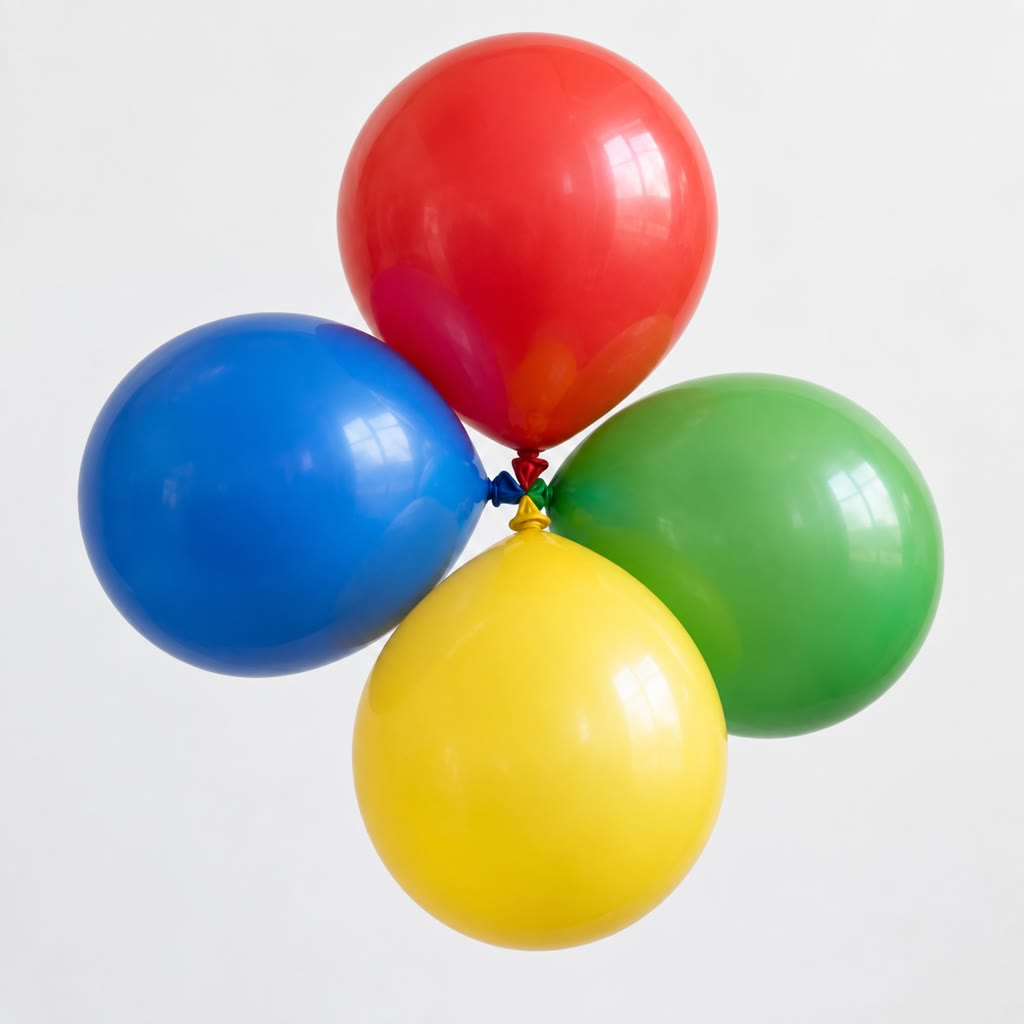
\includegraphics[width=0.38\linewidth]{images/book1/ai/g10-balloons-tetrahedron.jpg}

{\small Empat balon yang diikat bersama saling mendorong sejauh mungkin;
di dalam ruang, balon-balon itu mengarah ke sudut-sudut sebuah
tetrahedron, seperti keempat pasangan \omterm{def:g9:inside-the-atom:nucleus}{elektron} di sekeliling \omterm{def:g7:atoms-and-molecules:atom}{atom}
karbon.}
\end{omfigure}

\section{Menggambar molekul dalam ruang}

\begin{notation}[Baji pejal dan baji putus-putus]\label{not:g10:lewis-and-shape:wedge}
Untuk menggambar \omterm{def:g7:atoms-and-molecules:molecule}{molekul} dalam ruang di atas kertas datar, ikatan yang
terletak pada bidang kertas digambar sebagai garis biasa, ikatan yang
mengarah ke pembaca sebagai baji pejal, dan ikatan yang menjauhi pembaca
sebagai baji putus-putus. Metana lalu digambar seperti di bawah ini: dua
ikatan pada bidang kertas, satu ke arah pembaca dan satu menjauhinya.
\begin{center}
\chemfig{C(-[2]H)(-[4]H)(<[7]H)(<:[5]H)}
\end{center}
\end{notation}

\section{Latihan}

\begin{exercise}[$\star$]\label{exo:g10:lewis-and-shape:1}
Apa itu \omterm{def:g10:lewis-and-shape:covalent-bond}{ikatan kovalen}? Apa itu \omterm{def:g10:lewis-and-shape:lone-pair}{pasangan elektron bebas}?
\end{exercise}

\begin{exercise}[$\star$]\label{exo:g10:lewis-and-shape:2}
Berapa \omterm{def:g10:lewis-and-shape:covalent-bond}{ikatan kovalen} yang biasanya dibentuk hidrogen, karbon, nitrogen,
dan oksigen? Jelaskan dengan \omterm{def:g10:electron-shells:octet}{aturan oktet} dan \omterm{def:g10:electron-shells:octet}{aturan duplet}.
\end{exercise}

\begin{exercise}[$\star$]\label{exo:g10:lewis-and-shape:3}
Gambarlah \omterm{def:g10:lewis-and-shape:lewis-structure}{struktur Lewis} hidrogen klorida, \ce{HCl}, lalu hitung
\omterm{def:g9:inside-the-atom:nucleus}{elektron} di sekeliling klorin.
\end{exercise}

\begin{exercise}[$\star$]\label{exo:g10:lewis-and-shape:4}
Berapa \omterm{def:g10:electron-shells:valence}{elektron valensi} seluruhnya yang dimiliki \omterm{def:g7:atoms-and-molecules:molecule}{molekul} \ce{NH3}?
Berapa pasang?
\end{exercise}

\begin{exercise}[$\star$]\label{exo:g10:lewis-and-shape:5}
Sebutkan bentuk \ce{CH4}, \ce{NH3}, \ce{H2O}, dan \ce{CO2}.
\end{exercise}

\begin{exercise}[$\star\star$]\label{exo:g10:lewis-and-shape:6}
Gambarlah \omterm{def:g10:lewis-and-shape:lewis-structure}{struktur Lewis} hidrogen sulfida, \ce{H2S} (belerang segolongan
dengan oksigen), dan ramalkan bentuknya.
\end{exercise}

\begin{exercise}[$\star\star$]\label{exo:g10:lewis-and-shape:7}
Gambarlah \omterm{def:g10:lewis-and-shape:lewis-structure}{struktur Lewis} nitrogen, \ce{N2}, dengan mengikuti metode itu
langkah demi langkah.
\end{exercise}

\begin{exercise}[$\star\star$]\label{exo:g10:lewis-and-shape:8}
Gambarlah \omterm{def:g10:lewis-and-shape:lewis-structure}{struktur Lewis} metanol, \ce{CH3OH}, dan sebutkan bentuk di
sekeliling karbon dan di sekeliling oksigen.
\end{exercise}

\begin{exercise}[$\star\star$]\label{exo:g10:lewis-and-shape:9}
Mengapa \ce{CO2} linear dan \ce{H2O} bengkok, padahal keduanya memiliki
\omterm{def:g7:atoms-and-molecules:atom}{atom} pusat yang terhubung dengan dua \omterm{def:g7:atoms-and-molecules:atom}{atom} lain?
\end{exercise}

\begin{exercise}[$\star\star$]\label{exo:g10:lewis-and-shape:10}
Gambarlah \omterm{def:g10:lewis-and-shape:lewis-structure}{struktur Lewis} etena, \ce{C2H4}, dan sebutkan bentuk di
sekeliling setiap \omterm{def:g7:atoms-and-molecules:atom}{atom} karbon.
\end{exercise}

\begin{exercise}[$\star\star$]\label{exo:g10:lewis-and-shape:11}
Gambarlah \omterm{def:g10:lewis-and-shape:lewis-structure}{struktur Lewis} tetraklorometana, \ce{CCl4}, dan ramalkan
bentuknya.
\end{exercise}

\begin{exercise}[$\star\star\star$]\label{exo:g10:lewis-and-shape:12}
Dua \omterm{def:g7:atoms-and-molecules:molecule}{molekul} memiliki rumus \ce{C2H6O}. Gambarlah \omterm{def:g10:lewis-and-shape:lewis-structure}{struktur Lewis} untuk
masing-masing (yang satu memiliki ikatan O--H, yang lain rantai C--O--C).
\end{exercise}

\begin{exercise}[$\star\star\star$]\label{exo:g10:lewis-and-shape:13}
Jelaskan, dengan \omterm{def:g10:lewis-and-shape:lone-pair}{pasangan bebas}, mengapa sudut pada amonia (\ang{106.7})
lebih kecil daripada pada metana (\ang{109.5}), dan pada air
(\ang{104.5}) lebih kecil lagi.
\end{exercise}

\begin{exercise}[$\star\star\star$]\label{exo:g10:lewis-and-shape:14}
Gambarlah \omterm{def:g10:lewis-and-shape:lewis-structure}{struktur Lewis} hidrogen sianida, \ce{HCN}, dan metanal,
\ce{CH2O}, lalu sebutkan bentuknya.
\end{exercise}

\begin{exercise}[$\star\star\star$]\label{exo:g10:lewis-and-shape:15}
Ozon, \ce{O3}, adalah rantai tiga \omterm{def:g7:atoms-and-molecules:atom}{atom} oksigen. Hitung banyaknya
pasangan valensinya dan gambarlah sebuah \omterm{def:g10:lewis-and-shape:lewis-structure}{struktur Lewis} yang setiap
oksigennya memiliki oktet (satu \omterm{def:g10:lewis-and-shape:multiple-bond}{ikatan rangkap dua}, satu ikatan
tunggal). Ramalkan apakah \omterm{def:g7:atoms-and-molecules:molecule}{molekul} itu linear atau bengkok.
\end{exercise}

\section{Soal: Sebuah Molekul di dalam Kubus}

\begin{problem}[{Soal akhir pekan --- merancang bola-bola karbon sebuah
perangkat model molekul: pada sudut berapa lubang-lubangnya harus dibor?}]
\label{pb:g10:lewis-and-shape:1}
% ledger: ang:H2O, ang:NH3
Sebuah perusahaan membuat perangkat model \omterm{def:g7:atoms-and-molecules:molecule}{molekul}. Bola-bola karbon yang
hitam harus memiliki empat lubang, agar metana, etana, dan \omterm{def:g7:atoms-and-molecules:molecule}{molekul-molekul}
karbon lainnya terbentuk dengan bentuk yang benar. Sang insinyur memakai
sebuah siasat: sebuah tetrahedron beraturan pas di dalam sebuah kubus,
keempat titik sudutnya berada pada empat titik sudut kubus, dan tidak ada
dua di antaranya pada rusuk yang sama.

\medskip
\noindent\textbf{Bagian I --- \omterm{def:g10:lewis-and-shape:lewis-structure}{Struktur Lewis}.}
\begin{enumerate}
  \item Gambarlah \omterm{def:g10:lewis-and-shape:lewis-structure}{struktur Lewis} metana \ce{CH4}, amonia \ce{NH3}, dan
        air \ce{H2O}.
  \item Berapa kelompok \omterm{def:g9:inside-the-atom:nucleus}{elektron} yang mengelilingi \omterm{def:g7:atoms-and-molecules:atom}{atom} pusat pada
        masing-masing?
  \item Berapa di antaranya yang berupa \omterm{def:g10:lewis-and-shape:lone-pair}{pasangan bebas}?
  \item Mengapa bola karbon memerlukan empat lubang, sedangkan bola
        oksigen (untuk air) hanya dua?
  \item Model etana, \ce{C2H6}, memakai dua bola karbon. Gambarlah
        \omterm{def:g10:lewis-and-shape:lewis-structure}{struktur Lewis-nya}. Berapa tongkat yang menghubungkan kedua bola
        karbon, dan berapa bola hidrogen yang diperlukan?
\end{enumerate}

\medskip
\noindent\textbf{Bagian II --- Bentuk.}
\begin{enumerate}[resume]
  \item Sebutkan bentuk masing-masing ketiga \omterm{def:g7:atoms-and-molecules:molecule}{molekul} itu.
  \item Sudut yang terukur adalah \ang{106.7} pada amonia dan
        \ang{104.5} pada air. Jelaskan mengapa sudut-sudut itu lebih kecil
        daripada sudut pada metana.
  \item Mengapa bola oksigen untuk air tidak bisa sekadar berupa bola
        karbon dengan dua lubang yang dibiarkan kosong, jika perangkat itu
        harus memperlihatkan sudut yang sebenarnya?
  \item Pada karbon dioksida, \omterm{def:g7:atoms-and-molecules:atom}{atom} karbon membentuk dua \omterm{def:g10:lewis-and-shape:multiple-bond}{ikatan rangkap
        dua}. Sudut berapa yang harus memisahkan keduanya dalam model?
\end{enumerate}

\medskip
\noindent\textbf{Bagian III --- Kubusnya.}
Ambillah sebuah kubus dengan rusuk $a$. \omterm{def:g7:atoms-and-molecules:atom}{Atom} karbon berada di pusatnya;
keempat \omterm{def:g7:atoms-and-molecules:atom}{atom} hidrogen berada pada empat titik sudut kubus, tidak ada dua
di antaranya pada rusuk yang sama.
\begin{enumerate}[resume]
  \item Tunjukkan bahwa setiap dua \omterm{def:g7:atoms-and-molecules:atom}{atom} hidrogen ini berada di kedua ujung
        sebuah diagonal sisi kubus. Dengan teorema Pythagoras, hitung jarak
        antara keduanya dalam $a$.
  \item Diagonal ruang kubus (dari satu titik sudut ke titik sudut di
        seberangnya) panjangnya $a\sqrt{3}$. Simpulkan jarak dari \omterm{def:g7:atoms-and-molecules:atom}{atom}
        karbon ke sebuah \omterm{def:g7:atoms-and-molecules:atom}{atom} hidrogen.
  \item Ambillah $a = \qty{1}{cm}$ dalam sebuah model: berikan kedua
        jarak itu dalam sentimeter, sampai dua angka di belakang koma.
  \item Mengapa keempat jarak C--H sama?
\end{enumerate}

\medskip
\noindent\textbf{Bagian IV --- Sudutnya.}
\omterm{def:g7:atoms-and-molecules:atom}{Atom} karbon C dan dua \omterm{def:g7:atoms-and-molecules:atom}{atom} hidrogen H$_1$, H$_2$ membentuk segitiga sama
kaki. Misalkan M titik tengah H$_1$H$_2$.
\begin{enumerate}[resume]
  \item Jelaskan mengapa segitiga C\,M\,H$_1$ siku-siku di M.
  \item Hitung, dalam segitiga siku-siku ini, sinus sudut
        $\widehat{\text{M\,C\,H}_1}$, yaitu setengah sudut H--C--H.
  \item Simpulkan setengah sudut itu, lalu sudut H--C--H, sampai satu
        angka di belakang koma.
  \item Bandingkan dengan sudut pada tabel dalam bab ini.
  \item Nyatakan sudut yang harus dipakai untuk mengebor lubang-lubang
        sebuah bola karbon.
\end{enumerate}
\end{problem}
